\hypertarget{_lgm___a_e8___a_p8_8h}{
\section{/home/mgh/LanlGeoMag/libLanlGeoMag/Lgm/Lgm\_\-AE8\_\-AP8.h File Reference}
\label{_lgm___a_e8___a_p8_8h}\index{/home/mgh/LanlGeoMag/libLanlGeoMag/Lgm/Lgm\_\-AE8\_\-AP8.h@{/home/mgh/LanlGeoMag/libLanlGeoMag/Lgm/Lgm\_\-AE8\_\-AP8.h}}
}


This graph shows which files directly or indirectly include this file:\nopagebreak
\begin{figure}[H]
\begin{center}
\leavevmode
\includegraphics[width=167pt]{_lgm___a_e8___a_p8_8h__dep__incl}
\end{center}
\end{figure}
\subsection*{Defines}
\begin{CompactItemize}
\item 
\#define \hyperlink{_lgm___a_e8___a_p8_8h_f6fe3539bc85b26cfe03c522ae9a8c4a}{LGM\_\-AP8MAX}~1
\item 
\#define \hyperlink{_lgm___a_e8___a_p8_8h_ff4d10b0921ebff1fe69c04d4e54e14b}{LGM\_\-AP8MIN}~2
\item 
\#define \hyperlink{_lgm___a_e8___a_p8_8h_c6e048f3900fcc35c59bb8e9af0efd3f}{LGM\_\-AE8MAX}~7
\item 
\#define \hyperlink{_lgm___a_e8___a_p8_8h_4cbd010f780cb1d6137b51dc660eef49}{LGM\_\-AE8MIN}~8
\item 
\#define \hyperlink{_lgm___a_e8___a_p8_8h_387b8fb01026b7f305e3fa12b645f1fa}{LGM\_\-INTEGRAL\_\-FLUX}~1
\item 
\#define \hyperlink{_lgm___a_e8___a_p8_8h_c88bd45be8a1fcc073fbf7b21a92c1a5}{LGM\_\-DIFFERENTIAL\_\-FLUX}~2
\end{CompactItemize}
\subsection*{Functions}
\begin{CompactItemize}
\item 
void \hyperlink{_lgm___a_e8___a_p8_8h_c2047b8474f525b0c563986fb269a80a}{TRARA1} (int DESCR\mbox{[}$\,$\mbox{]}, int MAP\mbox{[}$\,$\mbox{]}, double FL, double BB0, double E\mbox{[}$\,$\mbox{]}, double F\mbox{[}$\,$\mbox{]}, int N)
\item 
double \hyperlink{_lgm___a_e8___a_p8_8h_2fe398897be76d62798262cceed6a432}{TRARA2} (int MAP\mbox{[}$\,$\mbox{]}, int IL, int IB, double FISTEP)
\item 
double \hyperlink{_lgm___a_e8___a_p8_8h_608555319590586b9fa28802d7a51628}{Lgm\_\-AE8\_\-AP8\_\-Flux} (double L, double BB0, int MODEL, int FLUXTYPE, double E1, double E2)
\item 
double \hyperlink{_lgm___a_e8___a_p8_8h_808d4c429cd0ffef1b3650491f20cc72}{Lgm\_\-AE8\_\-AP8\_\-FluxFromPos} (\hyperlink{struct_lgm___vector}{Lgm\_\-Vector} $\ast$u, int MODEL, int FLUXTYPE, double E1, double E2, \hyperlink{struct_lgm___mag_model_info}{Lgm\_\-MagModelInfo} $\ast$m)
\end{CompactItemize}


\subsection{Define Documentation}
\hypertarget{_lgm___a_e8___a_p8_8h_f6fe3539bc85b26cfe03c522ae9a8c4a}{
\index{Lgm\_\-AE8\_\-AP8.h@{Lgm\_\-AE8\_\-AP8.h}!LGM\_\-AP8MAX@{LGM\_\-AP8MAX}}
\index{LGM\_\-AP8MAX@{LGM\_\-AP8MAX}!Lgm_AE8_AP8.h@{Lgm\_\-AE8\_\-AP8.h}}
\subsubsection[{LGM\_\-AP8MAX}]{\setlength{\rightskip}{0pt plus 5cm}\#define LGM\_\-AP8MAX~1}}
\label{_lgm___a_e8___a_p8_8h_f6fe3539bc85b26cfe03c522ae9a8c4a}




Definition at line 16 of file Lgm\_\-AE8\_\-AP8.h.\hypertarget{_lgm___a_e8___a_p8_8h_ff4d10b0921ebff1fe69c04d4e54e14b}{
\index{Lgm\_\-AE8\_\-AP8.h@{Lgm\_\-AE8\_\-AP8.h}!LGM\_\-AP8MIN@{LGM\_\-AP8MIN}}
\index{LGM\_\-AP8MIN@{LGM\_\-AP8MIN}!Lgm_AE8_AP8.h@{Lgm\_\-AE8\_\-AP8.h}}
\subsubsection[{LGM\_\-AP8MIN}]{\setlength{\rightskip}{0pt plus 5cm}\#define LGM\_\-AP8MIN~2}}
\label{_lgm___a_e8___a_p8_8h_ff4d10b0921ebff1fe69c04d4e54e14b}




Definition at line 17 of file Lgm\_\-AE8\_\-AP8.h.\hypertarget{_lgm___a_e8___a_p8_8h_c6e048f3900fcc35c59bb8e9af0efd3f}{
\index{Lgm\_\-AE8\_\-AP8.h@{Lgm\_\-AE8\_\-AP8.h}!LGM\_\-AE8MAX@{LGM\_\-AE8MAX}}
\index{LGM\_\-AE8MAX@{LGM\_\-AE8MAX}!Lgm_AE8_AP8.h@{Lgm\_\-AE8\_\-AP8.h}}
\subsubsection[{LGM\_\-AE8MAX}]{\setlength{\rightskip}{0pt plus 5cm}\#define LGM\_\-AE8MAX~7}}
\label{_lgm___a_e8___a_p8_8h_c6e048f3900fcc35c59bb8e9af0efd3f}




Definition at line 18 of file Lgm\_\-AE8\_\-AP8.h.\hypertarget{_lgm___a_e8___a_p8_8h_4cbd010f780cb1d6137b51dc660eef49}{
\index{Lgm\_\-AE8\_\-AP8.h@{Lgm\_\-AE8\_\-AP8.h}!LGM\_\-AE8MIN@{LGM\_\-AE8MIN}}
\index{LGM\_\-AE8MIN@{LGM\_\-AE8MIN}!Lgm_AE8_AP8.h@{Lgm\_\-AE8\_\-AP8.h}}
\subsubsection[{LGM\_\-AE8MIN}]{\setlength{\rightskip}{0pt plus 5cm}\#define LGM\_\-AE8MIN~8}}
\label{_lgm___a_e8___a_p8_8h_4cbd010f780cb1d6137b51dc660eef49}




Definition at line 19 of file Lgm\_\-AE8\_\-AP8.h.\hypertarget{_lgm___a_e8___a_p8_8h_387b8fb01026b7f305e3fa12b645f1fa}{
\index{Lgm\_\-AE8\_\-AP8.h@{Lgm\_\-AE8\_\-AP8.h}!LGM\_\-INTEGRAL\_\-FLUX@{LGM\_\-INTEGRAL\_\-FLUX}}
\index{LGM\_\-INTEGRAL\_\-FLUX@{LGM\_\-INTEGRAL\_\-FLUX}!Lgm_AE8_AP8.h@{Lgm\_\-AE8\_\-AP8.h}}
\subsubsection[{LGM\_\-INTEGRAL\_\-FLUX}]{\setlength{\rightskip}{0pt plus 5cm}\#define LGM\_\-INTEGRAL\_\-FLUX~1}}
\label{_lgm___a_e8___a_p8_8h_387b8fb01026b7f305e3fa12b645f1fa}




Definition at line 20 of file Lgm\_\-AE8\_\-AP8.h.\hypertarget{_lgm___a_e8___a_p8_8h_c88bd45be8a1fcc073fbf7b21a92c1a5}{
\index{Lgm\_\-AE8\_\-AP8.h@{Lgm\_\-AE8\_\-AP8.h}!LGM\_\-DIFFERENTIAL\_\-FLUX@{LGM\_\-DIFFERENTIAL\_\-FLUX}}
\index{LGM\_\-DIFFERENTIAL\_\-FLUX@{LGM\_\-DIFFERENTIAL\_\-FLUX}!Lgm_AE8_AP8.h@{Lgm\_\-AE8\_\-AP8.h}}
\subsubsection[{LGM\_\-DIFFERENTIAL\_\-FLUX}]{\setlength{\rightskip}{0pt plus 5cm}\#define LGM\_\-DIFFERENTIAL\_\-FLUX~2}}
\label{_lgm___a_e8___a_p8_8h_c88bd45be8a1fcc073fbf7b21a92c1a5}




Definition at line 21 of file Lgm\_\-AE8\_\-AP8.h.

\subsection{Function Documentation}
\hypertarget{_lgm___a_e8___a_p8_8h_c2047b8474f525b0c563986fb269a80a}{
\index{Lgm\_\-AE8\_\-AP8.h@{Lgm\_\-AE8\_\-AP8.h}!TRARA1@{TRARA1}}
\index{TRARA1@{TRARA1}!Lgm_AE8_AP8.h@{Lgm\_\-AE8\_\-AP8.h}}
\subsubsection[{TRARA1}]{\setlength{\rightskip}{0pt plus 5cm}void TRARA1 (int {\em DESCR}\mbox{[}$\,$\mbox{]}, \/  int {\em MAP}\mbox{[}$\,$\mbox{]}, \/  double {\em FL}, \/  double {\em BB0}, \/  double {\em E}\mbox{[}$\,$\mbox{]}, \/  double {\em F}\mbox{[}$\,$\mbox{]}, \/  int {\em N})}}
\label{_lgm___a_e8___a_p8_8h_c2047b8474f525b0c563986fb269a80a}




Definition at line 5357 of file Lgm\_\-AE8\_\-AP8.c.

Here is the call graph for this function:\nopagebreak
\begin{figure}[H]
\begin{center}
\leavevmode
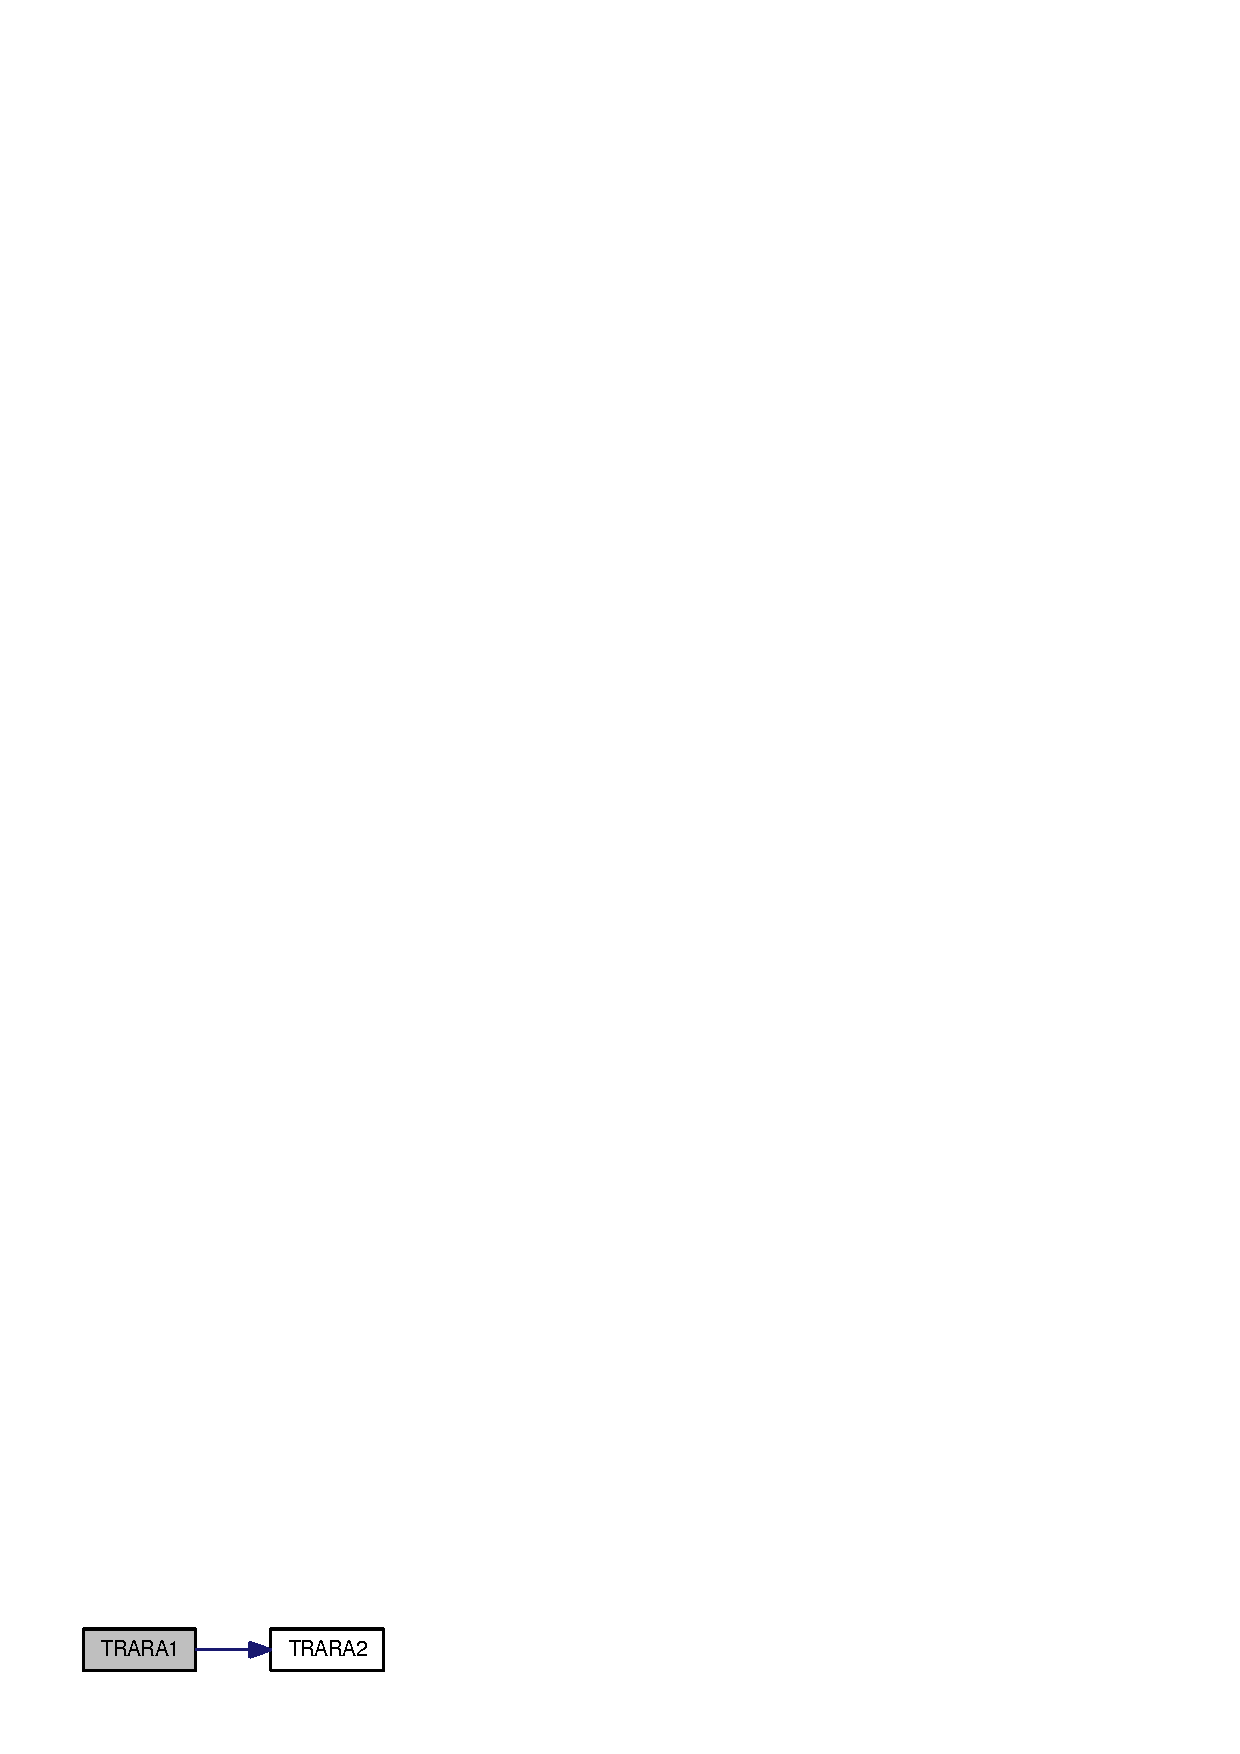
\includegraphics[width=94pt]{_lgm___a_e8___a_p8_8h_c2047b8474f525b0c563986fb269a80a_cgraph}
\end{center}
\end{figure}


Here is the caller graph for this function:\nopagebreak
\begin{figure}[H]
\begin{center}
\leavevmode
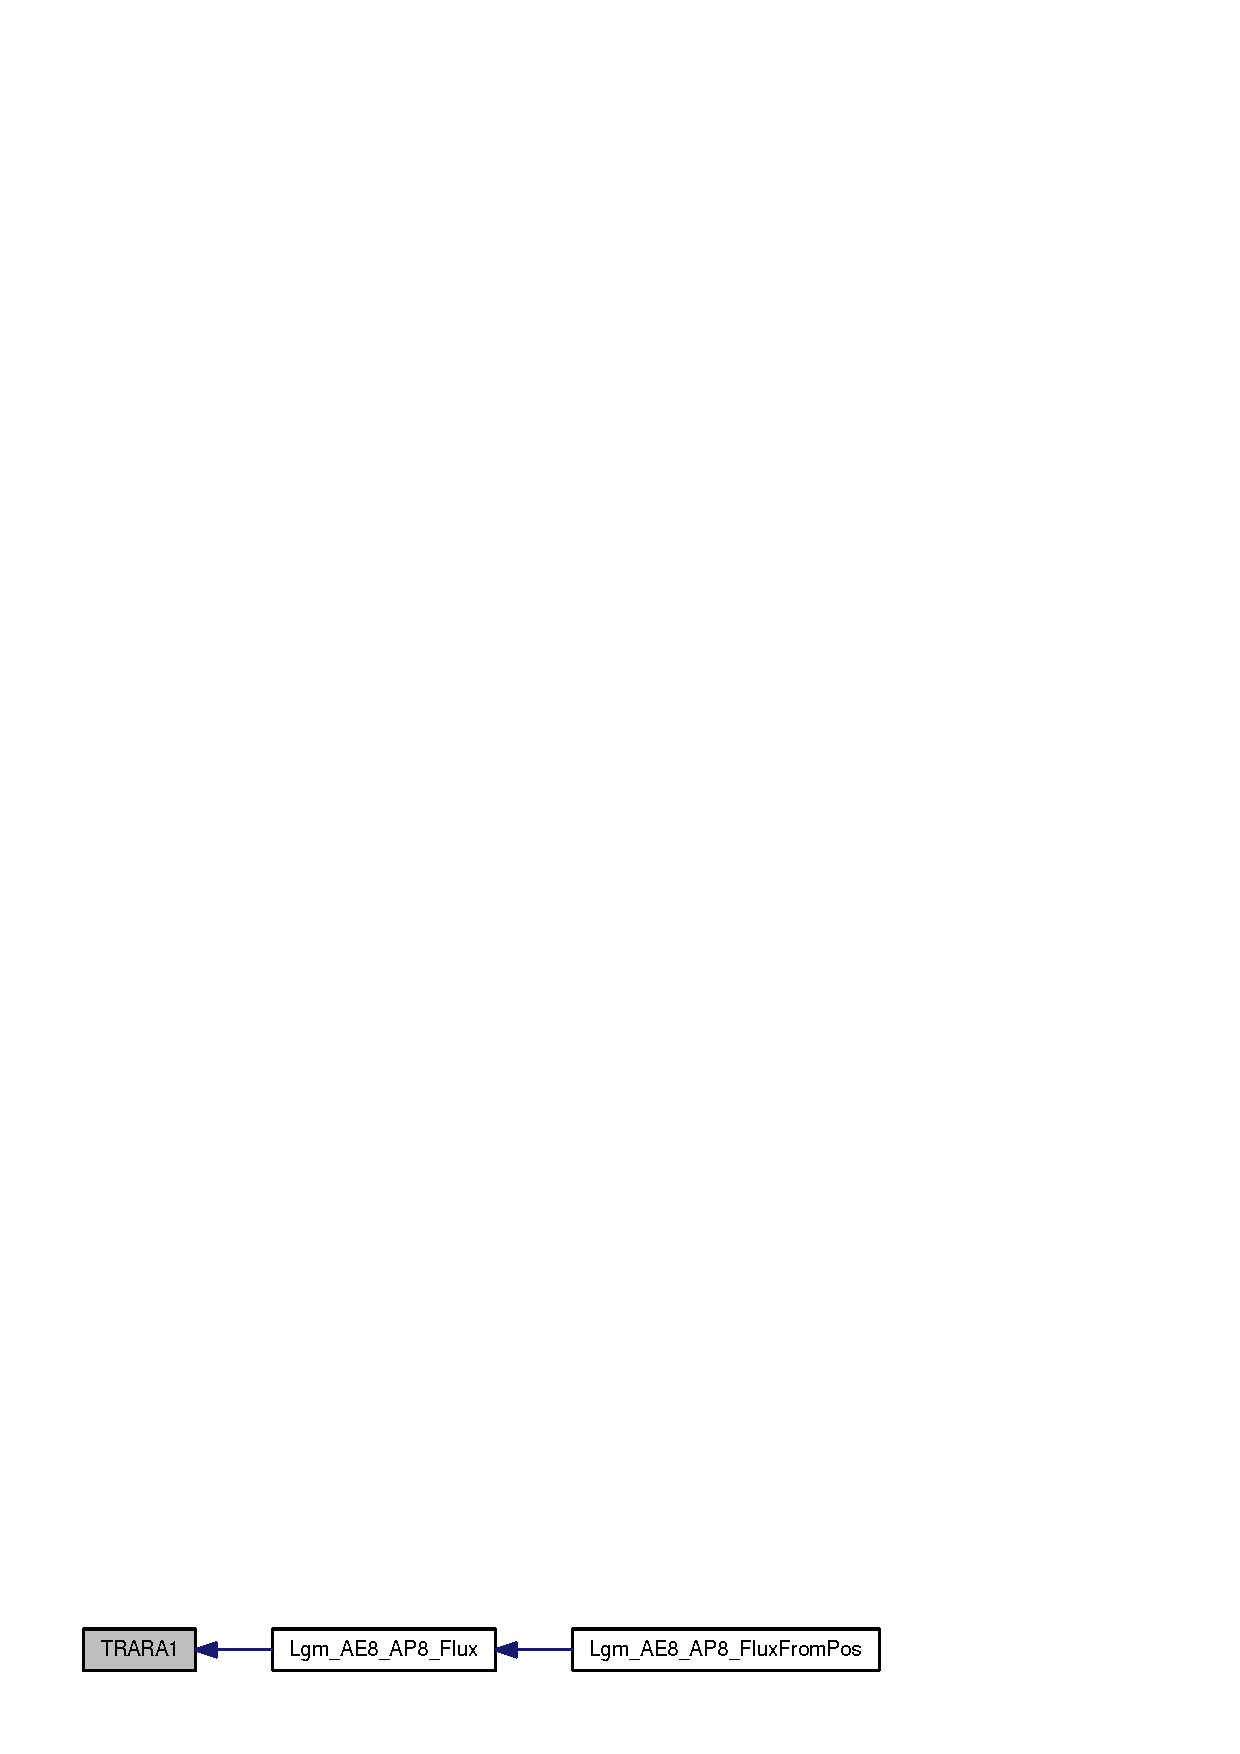
\includegraphics[width=213pt]{_lgm___a_e8___a_p8_8h_c2047b8474f525b0c563986fb269a80a_icgraph}
\end{center}
\end{figure}
\hypertarget{_lgm___a_e8___a_p8_8h_2fe398897be76d62798262cceed6a432}{
\index{Lgm\_\-AE8\_\-AP8.h@{Lgm\_\-AE8\_\-AP8.h}!TRARA2@{TRARA2}}
\index{TRARA2@{TRARA2}!Lgm_AE8_AP8.h@{Lgm\_\-AE8\_\-AP8.h}}
\subsubsection[{TRARA2}]{\setlength{\rightskip}{0pt plus 5cm}double TRARA2 (int {\em MAP}\mbox{[}$\,$\mbox{]}, \/  int {\em IL}, \/  int {\em IB}, \/  double {\em FISTEP})}}
\label{_lgm___a_e8___a_p8_8h_2fe398897be76d62798262cceed6a432}




Definition at line 5464 of file Lgm\_\-AE8\_\-AP8.c.

Here is the caller graph for this function:\nopagebreak
\begin{figure}[H]
\begin{center}
\leavevmode
\includegraphics[width=258pt]{_lgm___a_e8___a_p8_8h_2fe398897be76d62798262cceed6a432_icgraph}
\end{center}
\end{figure}
\hypertarget{_lgm___a_e8___a_p8_8h_608555319590586b9fa28802d7a51628}{
\index{Lgm\_\-AE8\_\-AP8.h@{Lgm\_\-AE8\_\-AP8.h}!Lgm\_\-AE8\_\-AP8\_\-Flux@{Lgm\_\-AE8\_\-AP8\_\-Flux}}
\index{Lgm\_\-AE8\_\-AP8\_\-Flux@{Lgm\_\-AE8\_\-AP8\_\-Flux}!Lgm_AE8_AP8.h@{Lgm\_\-AE8\_\-AP8.h}}
\subsubsection[{Lgm\_\-AE8\_\-AP8\_\-Flux}]{\setlength{\rightskip}{0pt plus 5cm}double Lgm\_\-AE8\_\-AP8\_\-Flux (double {\em L}, \/  double {\em BB0}, \/  int {\em MODEL}, \/  int {\em FLUXTYPE}, \/  double {\em E1}, \/  double {\em E2})}}
\label{_lgm___a_e8___a_p8_8h_608555319590586b9fa28802d7a51628}




Definition at line 5155 of file Lgm\_\-AE8\_\-AP8.c.

Here is the call graph for this function:\nopagebreak
\begin{figure}[H]
\begin{center}
\leavevmode
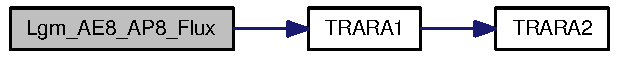
\includegraphics[width=166pt]{_lgm___a_e8___a_p8_8h_608555319590586b9fa28802d7a51628_cgraph}
\end{center}
\end{figure}


Here is the caller graph for this function:\nopagebreak
\begin{figure}[H]
\begin{center}
\leavevmode
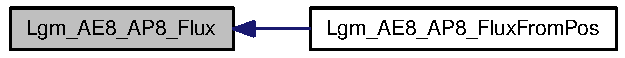
\includegraphics[width=168pt]{_lgm___a_e8___a_p8_8h_608555319590586b9fa28802d7a51628_icgraph}
\end{center}
\end{figure}
\hypertarget{_lgm___a_e8___a_p8_8h_808d4c429cd0ffef1b3650491f20cc72}{
\index{Lgm\_\-AE8\_\-AP8.h@{Lgm\_\-AE8\_\-AP8.h}!Lgm\_\-AE8\_\-AP8\_\-FluxFromPos@{Lgm\_\-AE8\_\-AP8\_\-FluxFromPos}}
\index{Lgm\_\-AE8\_\-AP8\_\-FluxFromPos@{Lgm\_\-AE8\_\-AP8\_\-FluxFromPos}!Lgm_AE8_AP8.h@{Lgm\_\-AE8\_\-AP8.h}}
\subsubsection[{Lgm\_\-AE8\_\-AP8\_\-FluxFromPos}]{\setlength{\rightskip}{0pt plus 5cm}double Lgm\_\-AE8\_\-AP8\_\-FluxFromPos ({\bf Lgm\_\-Vector} $\ast$ {\em u}, \/  int {\em MODEL}, \/  int {\em FLUXTYPE}, \/  double {\em E1}, \/  double {\em E2}, \/  {\bf Lgm\_\-MagModelInfo} $\ast$ {\em m})}}
\label{_lgm___a_e8___a_p8_8h_808d4c429cd0ffef1b3650491f20cc72}




Definition at line 5701 of file Lgm\_\-AE8\_\-AP8.c.

Here is the call graph for this function:\nopagebreak
\begin{figure}[H]
\begin{center}
\leavevmode
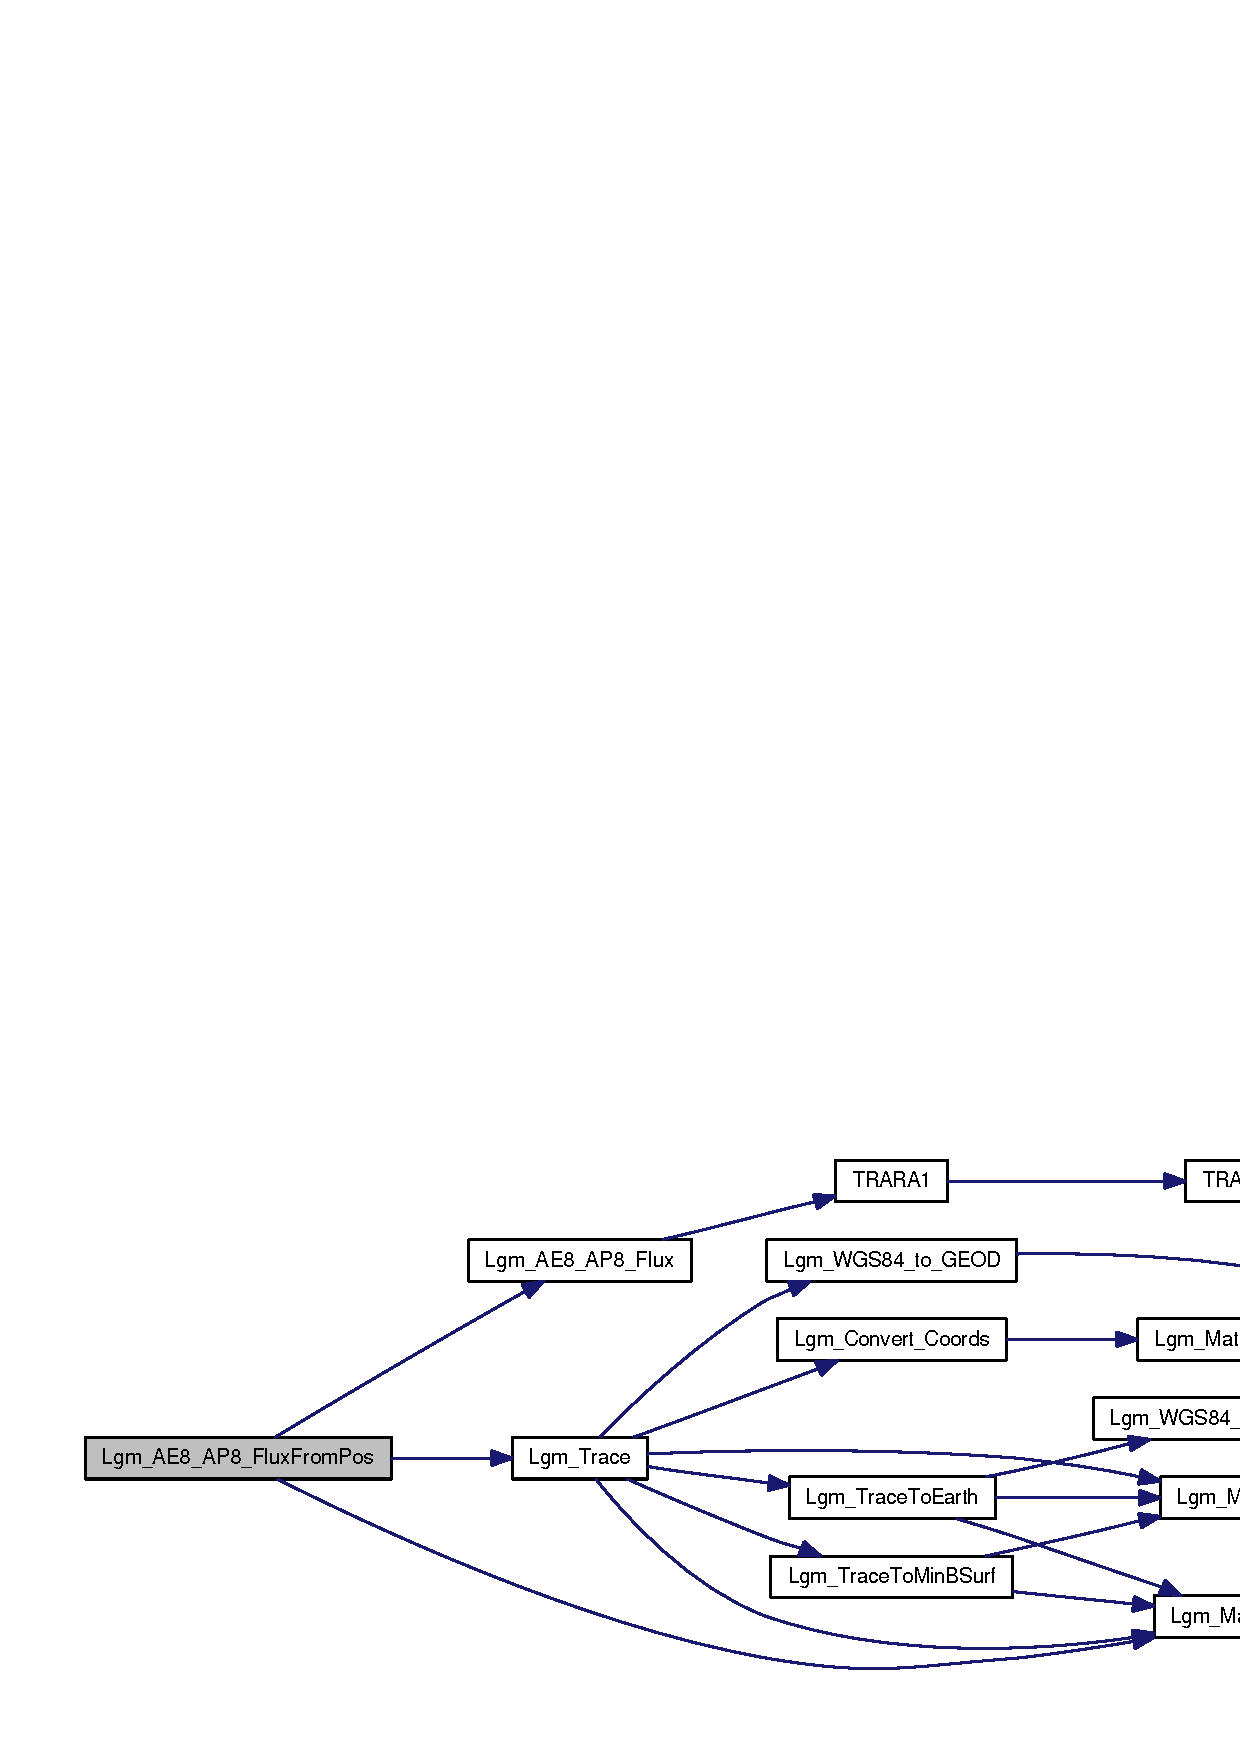
\includegraphics[width=420pt]{_lgm___a_e8___a_p8_8h_808d4c429cd0ffef1b3650491f20cc72_cgraph}
\end{center}
\end{figure}
